\documentclass[
  man,
  floatsintext,
  longtable,
  nolmodern,
  notxfonts,
  notimes,
  colorlinks=true,linkcolor=blue,citecolor=blue,urlcolor=blue]{apa7}

\usepackage{amsmath}
\usepackage{amssymb}




\RequirePackage{longtable}
\RequirePackage{threeparttablex}

\makeatletter
\renewcommand{\paragraph}{\@startsection{paragraph}{4}{\parindent}%
	{0\baselineskip \@plus 0.2ex \@minus 0.2ex}%
	{-.5em}%
	{\normalfont\normalsize\bfseries\typesectitle}}

\renewcommand{\subparagraph}[1]{\@startsection{subparagraph}{5}{0.5em}%
	{0\baselineskip \@plus 0.2ex \@minus 0.2ex}%
	{-\z@\relax}%
	{\normalfont\normalsize\bfseries\itshape\hspace{\parindent}{#1}\textit{\addperi}}{\relax}}
\makeatother




\usepackage{longtable, booktabs, multirow, multicol, colortbl, hhline, caption, array, float, xpatch}
\setcounter{topnumber}{2}
\setcounter{bottomnumber}{2}
\setcounter{totalnumber}{4}
\renewcommand{\topfraction}{0.85}
\renewcommand{\bottomfraction}{0.85}
\renewcommand{\textfraction}{0.15}
\renewcommand{\floatpagefraction}{0.7}

\usepackage{tcolorbox}
\tcbuselibrary{listings,theorems, breakable, skins}
\usepackage{fontawesome5}

\definecolor{quarto-callout-color}{HTML}{909090}
\definecolor{quarto-callout-note-color}{HTML}{0758E5}
\definecolor{quarto-callout-important-color}{HTML}{CC1914}
\definecolor{quarto-callout-warning-color}{HTML}{EB9113}
\definecolor{quarto-callout-tip-color}{HTML}{00A047}
\definecolor{quarto-callout-caution-color}{HTML}{FC5300}
\definecolor{quarto-callout-color-frame}{HTML}{ACACAC}
\definecolor{quarto-callout-note-color-frame}{HTML}{4582EC}
\definecolor{quarto-callout-important-color-frame}{HTML}{D9534F}
\definecolor{quarto-callout-warning-color-frame}{HTML}{F0AD4E}
\definecolor{quarto-callout-tip-color-frame}{HTML}{02B875}
\definecolor{quarto-callout-caution-color-frame}{HTML}{FD7E14}

%\newlength\Oldarrayrulewidth
%\newlength\Oldtabcolsep


\usepackage{hyperref}




\providecommand{\tightlist}{%
  \setlength{\itemsep}{0pt}\setlength{\parskip}{0pt}}
\usepackage{longtable,booktabs,array}
\usepackage{calc} % for calculating minipage widths
% Correct order of tables after \paragraph or \subparagraph
\usepackage{etoolbox}
\makeatletter
\patchcmd\longtable{\par}{\if@noskipsec\mbox{}\fi\par}{}{}
\makeatother
% Allow footnotes in longtable head/foot
\IfFileExists{footnotehyper.sty}{\usepackage{footnotehyper}}{\usepackage{footnote}}
\makesavenoteenv{longtable}

\usepackage{graphicx}
\makeatletter
\newsavebox\pandoc@box
\newcommand*\pandocbounded[1]{% scales image to fit in text height/width
  \sbox\pandoc@box{#1}%
  \Gscale@div\@tempa{\textheight}{\dimexpr\ht\pandoc@box+\dp\pandoc@box\relax}%
  \Gscale@div\@tempb{\linewidth}{\wd\pandoc@box}%
  \ifdim\@tempb\p@<\@tempa\p@\let\@tempa\@tempb\fi% select the smaller of both
  \ifdim\@tempa\p@<\p@\scalebox{\@tempa}{\usebox\pandoc@box}%
  \else\usebox{\pandoc@box}%
  \fi%
}
% Set default figure placement to htbp
\def\fps@figure{htbp}
\makeatother


% definitions for citeproc citations
\NewDocumentCommand\citeproctext{}{}
\NewDocumentCommand\citeproc{mm}{%
  \begingroup\def\citeproctext{#2}\cite{#1}\endgroup}
\makeatletter
 % allow citations to break across lines
 \let\@cite@ofmt\@firstofone
 % avoid brackets around text for \cite:
 \def\@biblabel#1{}
 \def\@cite#1#2{{#1\if@tempswa , #2\fi}}
\makeatother
\newlength{\cslhangindent}
\setlength{\cslhangindent}{1.5em}
\newlength{\csllabelwidth}
\setlength{\csllabelwidth}{3em}
\newenvironment{CSLReferences}[2] % #1 hanging-indent, #2 entry-spacing
 {\begin{list}{}{%
  \setlength{\itemindent}{0pt}
  \setlength{\leftmargin}{0pt}
  \setlength{\parsep}{0pt}
  % turn on hanging indent if param 1 is 1
  \ifodd #1
   \setlength{\leftmargin}{\cslhangindent}
   \setlength{\itemindent}{-1\cslhangindent}
  \fi
  % set entry spacing
  \setlength{\itemsep}{#2\baselineskip}}}
 {\end{list}}
\usepackage{calc}
\newcommand{\CSLBlock}[1]{\hfill\break\parbox[t]{\linewidth}{\strut\ignorespaces#1\strut}}
\newcommand{\CSLLeftMargin}[1]{\parbox[t]{\csllabelwidth}{\strut#1\strut}}
\newcommand{\CSLRightInline}[1]{\parbox[t]{\linewidth - \csllabelwidth}{\strut#1\strut}}
\newcommand{\CSLIndent}[1]{\hspace{\cslhangindent}#1}





\usepackage{newtx}

\defaultfontfeatures{Scale=MatchLowercase}
\defaultfontfeatures[\rmfamily]{Ligatures=TeX,Scale=1}





\title{What's in a \(p\)-value?}


\shorttitle{What's in a \(p\)-value?}


\usepackage{etoolbox}









\authorsnames[{1,2},{2}]{Frederik Aust,Eric-Jan Wagenmakers}







\authorsaffiliations{
{University of Cologne},{University of Amsterdam}}




\leftheader{Aust and Wagenmakers}

\date{2025-02-28}


\abstract{\textbf{TODO} }

\keywords{p-values, evidence, Bayes factor}

\authornote{\par{\addORCIDlink{Frederik
Aust}{0000-0003-4900-788X}}\par{\addORCIDlink{Eric-Jan
Wagenmakers}{0000-0003-1596-1034}} 

\par{       }
\par{Correspondence concerning this article should be addressed to }
}

\makeatletter
\let\endoldlt\endlongtable
\def\endlongtable{
\hline
\endoldlt
}
\makeatother

\urlstyle{same}



\usepackage{booktabs}
\usepackage{caption}
\usepackage{longtable}
\usepackage{colortbl}
\usepackage{array}
\usepackage{anyfontsize}
\usepackage{multirow}
\makeatletter
\@ifpackageloaded{caption}{}{\usepackage{caption}}
\AtBeginDocument{%
\ifdefined\contentsname
  \renewcommand*\contentsname{Table of contents}
\else
  \newcommand\contentsname{Table of contents}
\fi
\ifdefined\listfigurename
  \renewcommand*\listfigurename{List of Figures}
\else
  \newcommand\listfigurename{List of Figures}
\fi
\ifdefined\listtablename
  \renewcommand*\listtablename{List of Tables}
\else
  \newcommand\listtablename{List of Tables}
\fi
\ifdefined\figurename
  \renewcommand*\figurename{Figure}
\else
  \newcommand\figurename{Figure}
\fi
\ifdefined\tablename
  \renewcommand*\tablename{Table}
\else
  \newcommand\tablename{Table}
\fi
}
\@ifpackageloaded{float}{}{\usepackage{float}}
\floatstyle{ruled}
\@ifundefined{c@chapter}{\newfloat{codelisting}{h}{lop}}{\newfloat{codelisting}{h}{lop}[chapter]}
\floatname{codelisting}{Listing}
\newcommand*\listoflistings{\listof{codelisting}{List of Listings}}
\makeatother
\makeatletter
\makeatother
\makeatletter
\@ifpackageloaded{caption}{}{\usepackage{caption}}
\@ifpackageloaded{subcaption}{}{\usepackage{subcaption}}
\makeatother

% From https://tex.stackexchange.com/a/645996/211326
%%% apa7 doesn't want to add appendix section titles in the toc
%%% let's make it do it
\makeatletter
\xpatchcmd{\appendix}
  {\par}
  {\addcontentsline{toc}{section}{\@currentlabelname}\par}
  {}{}
\makeatother

%% Disable longtable counter
%% https://tex.stackexchange.com/a/248395/211326

\usepackage{etoolbox}

\makeatletter
\patchcmd{\LT@caption}
  {\bgroup}
  {\bgroup\global\LTpatch@captiontrue}
  {}{}
\patchcmd{\longtable}
  {\par}
  {\par\global\LTpatch@captionfalse}
  {}{}
\apptocmd{\endlongtable}
  {\ifLTpatch@caption\else\addtocounter{table}{-1}\fi}
  {}{}
\newif\ifLTpatch@caption
\makeatother

\begin{document}

\maketitle

\hypertarget{toc}{}
\tableofcontents
\newpage
\section[Introduction]{What's in a \(p\)-value?}

\setcounter{secnumdepth}{5}

\setlength\LTleft{0pt}


Null hypothesis significance testing is ubiquitous in psychological
science and beyond. The key outcome of this statistical procedure is the
\(p\) value, which researchers routinely use to decide whether to reject
the null hypothesis \(\mathcal{H}_0\). It is common to interpret \(p\)
values as a measure of statistical evidence or as the implied
probability that \(\mathcal{H}_0\) is true
(\citeproc{ref-Cohen1994}{Cohen, 1994};
\citeproc{ref-Gigerenzer2018}{Gigerenzer, 2018}). This is despite
repeated efforts to explain that the \(p\) value is \emph{not} a measure
of evidence {[}\textbf{???}, Hubbard and Lindsay
(\citeproc{ref-Hubbard2008}{2008}); Royall, 1997; Goodman \& Royall,
1988{]}. In contrast, Bayesian model comparisons do yield a principled
measure of relative evidence: the Bayes factor. However, unlike \(p\)
values, the Bayes factor is not routinely reported. Fortunately for the
evidence-seeking reader, \(p\) values can be monotonically related to
the Bayes factor (\citeproc{ref-Berger1987}{Berger \& Sellke, 1987})
and, as we will show, this relationship can be exploited to gauge the
evidence implied by a reported \(p\) value. All that is needed is the
effective sample size (\citeproc{ref-Wagenmakers2022}{Wagenmakers,
2022}). The resulting approximate Bayes factor is a useful tool for
researchers, reviewers, and readers to interpret emprical results---even
under conditions that threaten frequentist inference, most notably when
the data may have been peaked at.

For those that unfamiliar with the debate, the upcoming section
illustrate practical problems that arise when \(p\) values are
interpreted as measures of evidence. In the following two sections, we
show that the Bayes factor avoids these problems because it quantifies
evidence as the relative predictive accuracy of two competing
hypotheses. We highlight two additional attractive properties of the
Bayes factor: Identifying weak or inconclusive evidence and the
independence of researchers' sampling intentions. Although we have doen
our best to make these section engaging, busy readers familiar with the
Bayes factor may wish to skip them. We then get to the heart of our
contribution: We show how the monotonic relationship between \(p\)
values and the Bayes factor can be exploited in a simple formula to
approximate the Bayes factor. This approximation combines \(p\) and
effective sample size \(n_\text{eff}\) and closely approximates the
Bayes factor. We demonstrate the closeness of the approximation by
reanalyzing two large datasets of published \(p\) values for tests of
mean comparisons and proportions. Finally, we discuss the implications
of the approximation for the suggested evidential interpretations of
\(p\) values.

\section{\texorpdfstring{\(p\) as conflict or
surprise}{p as conflict or surprise}}\label{p-as-conflict-or-surprise}

To understand why \(p\) values are not a measure of evidence, it may be
useful to briefly review what they are. In the following, we will limit
our discussion to one-sided \(p\)-values for the sake of simplicity. The
\(p\) value is defined as the percentile of the observed test statistic
\(t\) in the distribution of all test statistics \(T\) that could have
been observed if the null hypothesis \(\mathcal{H}_0\) were true,

\[
p = \text{Pr}(T \geq \text{abs}(t) \mid \mathcal{H}_0).
\]

In other words, the \(p\) value is measure of conflict between the data
and \(\mathcal{H}_0\) and quantifies the information against
\(\mathcal{H}_0\)---smaller values indicating stronger conflict
(\citeproc{ref-Greenland2019}{Greenland, 2019};
\citeproc{ref-Perezgonzalez2015}{Perezgonzalez, 2015}).

This conflict between the data and \(\mathcal{H}_0\) can be expressed on
a different scale: the \(s\) value, where \(s = -\log_2(p)\)
(\citeproc{ref-Rafi2020}{Rafi \& Greenland, 2020}). The \(s\) value can
be thought of as a measure of \emph{surprise} in units of bits (or
Shannon-information). To intuit the meaning of a bit of information,
indulge me in a game of chance: The rules are simple: I toss a coin;
tails, you win; heads, I win. Let's play. In the first round, I flip the
coin and it comes up heads. I flip the coin a second time and, again, it
comes up heads; the third and fourth time the coin also comes up heads.
Take a moment to imagine your surprise; hold on to that feeling.

Entering this game of chance, you hopefully assumed that the coin is
fair---who would try to cheat their readers. Based on this assumption
every subsequent flip that comes up heads should increase your surprise
about my run of good luck. The \(s\) value quantifies this surprise:
\(s = 2\) corresponds to a streak of all heads from two tosses,
\(s = 3\) to a streak of all heads from three tosses, and so on. The
surprise you felt after the fourth flip roughly corresponds to the
surprise conveyed by \(p = .05 = .5^{4.32}\) in an one-sided exact
binomail test (\citeproc{ref-Cole2020}{Cole et al., 2020}; p.~109,
\citeproc{ref-Greenland2019}{Greenland, 2019}). I flip the coin one last
time and, lo and behold, it comes up heads again.

Did I get lucky? Are you suspicious, yet? Am I using a flipping
technique that biases the coin to come up heads? The \(p\) value for
this run of five heads drops to \(p = .031 = 0.5^5\); adopting an error
rate of \(\alpha = .05\), which most scientific disciplines deem
acceptable, the surprise, that is the conflict between data and
\(\mathcal{H}_0:~\theta = .5\) is strong enough to reject
\(\mathcal{H}_0\) and conclude foul play on my part. But I will protest:
``This is preposterous! There is no evidence for such accusations. You
are jumping to conclusions!'' Well, what is the evidence? How strongly
should my run of good luck change your belief that I tossed the coin
fairly? Or, more formally, what is the posterior probability of
\(\mathcal{H}_0\) given the data \(\mathbf{y}\),
\(\text{Pr}(\mathcal{H}_0 \mid \mathbf{y} = \text{{HHHHH}})\)? To answer
these question, we need to think about alternatives to
\(\mathcal{H}_0\).

In the following section we attempt to convey an intuitve understanding
of the Bayes factor and illustrate how this measure of evidence differs
from the \(p\) value. This and the next section may leave some readers
wanting for a more in-depth treatment---we refer them to the annotated
reading list provided by Etz et al. (\citeproc{ref-Etz2017}{2017}; also
see \citeproc{ref-Allabadi2024}{Al-Labadi et al., 2024};
\citeproc{ref-Morey2016}{Morey et al., 2016}).

\section{Quantifying evidence}\label{quantifying-evidence}

Quantifying \(\text{Pr}(\mathcal{H}_0)\) requires that we distribute
probabilities over a finite number of hypotheses \(\mathcal{H}_i\), such
that \(\sum_i{\text{Pr}(\mathcal{H}_i)} = 1\). If no alternative to
\(\mathcal{H}_0\) exists, the posterior probability of \(\mathcal{H}_0\)
must be 1---regardless of the data. If there are alternatives but they
are not specified, \(\text{Pr}(\mathcal{H}_0)\) is undefined---we can
only quantify the surprise, i.e.~the conflict between the data and
\(\mathcal{H}_0\). But it remains unclear how to translate this surprise
into the probability that the coin was tossed fairly. We must specified
alternative hypotheses to derive the posterior probability,

\[
\text{Pr}(\mathcal{H}_0 \mid \mathbf{y}) =  \text{Pr}(\mathcal{H}_0) \times \frac{\text{Pr}(\mathbf{y} \mid \mathcal{H}_0)}{\sum_i{\text{Pr}(\mathcal{H}_i) \times \text{Pr}(\mathbf{y} \mid \mathcal{H}_i)}}.
\]

So let's think about alternatives to fair coin tossing. What's the
probability \(\theta\) of coming up heads for coin tossing tricksters?
Could I toss my coin to come up heads with a probability of
\(\theta = 1\) without youa noticing? The data seem to suggest that this
is the most likely alternative wiht \(\hat\theta = 5/5 = 1\). This would
be outrageous (but also impressive, no?), so let's entertain this
alternative hypothesis as \(\mathcal{H}_1\). Maybe I am a less skilled
or more subtle trickster, flipping my coin to come up heads with a
probability of \(\theta = .60\), \(\theta = .65\), or \(\theta = .70\)?
None of these exact probabilites seems to deserve special consideration.
All are plausible, some more than others; so we will specify a general
alternative hypothesis and assign \(\theta\) a prior distribution
constraining \(\theta > .5\),
\(\mathcal{H}_2:~2\theta-1 \sim \mathcal{B}(a = 2, b = 3)\), see
Figure~\ref{fig-coin-hypotheses}.

\begin{figure}

\caption{\label{fig-coin-hypotheses}Prior probability distributions for
the probability of heads \(\theta\) for the toss of a coin. The orange
arrow represents the point hypothesis \(\mathcal{H}_0\) that the coin is
fair, the purple arrow represents the point hypothesis \(\mathcal{H}_1\)
that the coin always comes up heads, and the red curve is the continuous
hypothesis \(\mathcal{H}_2\) that the coin is loaded to come up heads
but the probability of heads is unknown. The dashed line represents the
posterior distribution of \(\theta\) given \(\mathcal{H}_2\) and the
data \(\mathbf{y} = \{HHHHH\}\).}

\centering{

\pandocbounded{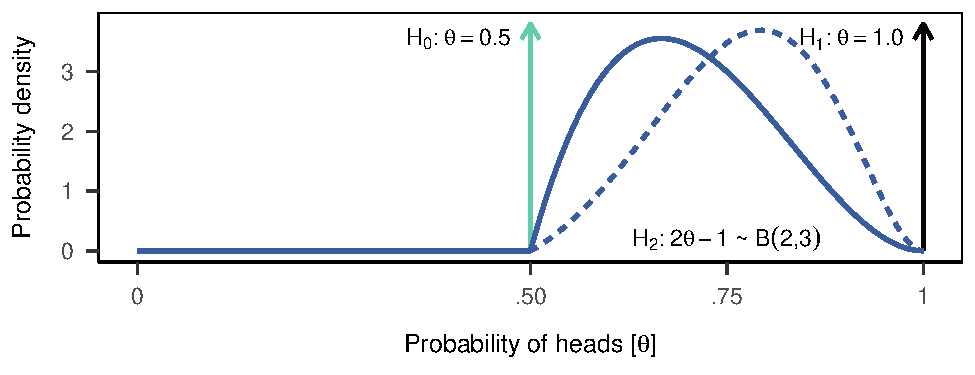
\includegraphics[keepaspectratio]{whats-in-a-p-value_files/figure-pdf/fig-coin-hypotheses-1.pdf}}

}

\end{figure}%

Deriving the posterior probability of \(\mathcal{H}_0\) directly is
conceptually inconvenient. Reasonable people will disagree what all
relevant alternatives are and how likely they are a priori. It is more
convenient to think about the odds of pairs of hypotheses and the
relative evidence in the data, i.e.~the Bayes factor (BF)
\(\text{BF}_{01}\):

\[
\underbrace{ \frac{p(\mathcal{H}_0  \mid \mathbf{y})}{p(\mathcal{H}_1  \mid \mathbf{y})}}_{\substack{\text{Posterior beliefs}\\ \text{about hypotheses}} } \,\, =
\underbrace{ \frac{p(\mathcal{H}_0)}{p(\mathcal{H}_1)}}_{\substack{\text{Prior beliefs}\\ \text{about hypotheses}} }
\times \,\,\,\,\,
\underbrace{ \frac{p(\mathbf{y} \mid \mathcal{H}_0)}{p(\mathbf{y} \mid  \mathcal{H}_1)}}_{\substack{\text{Bayes factor BF}_{01}\\(\text{relative evidence}) } }.
\]

On the odds scale, we can limit our considerations to two relevnt
hypotheses and it allows us to separate the prior beliefs from the
evidence in the data. Now it becomes clear that according to Bayes
theorem, evidence is defined as the relative predictive accuracy of two
hypotheses. The evidence quantifies how much better one hypothesis
predicts the data than another, or with under which hypothesis the data
are less surprising.

So, what's the evidence that I cheated you? As noted above, a run of
five heads corresponds to a \(p = .031 = 0.5^5\) and \(s = 5\) assuming
\(\mathcal{H}_0\) is true and \(\theta = .5\). Conveniently, I
constructed this example such that
\(\Pr(\mathbf{y} \mid \mathcal{H}_i) = \theta^5 = p\)---this is usually
not the case. This means that if \(\mathcal{H}_1\) is true and
\(\theta = 1\), \(\Pr(\mathbf{y} \mid \mathcal{H}_1) = 1\). Hence,
assuming that if I cheat it is literally \emph{impossible} for the coin
to come up tails, the data are strong evidence that I cheated you,
\(\text{BF}_{10} = 1/p = 1/.031 = 32\),
Table~\ref{tbl-evidence-categories}.

Attentive readers may now point out that, counter to our initial claims,
\(p = 1/\text{BF}_{10} = \text{BF}_{01}\) \emph{is} a measure of
evidence against \(\mathcal{H}_0\)---if we assume that \(\mathcal{H}_1\)
is the relavant alternative hypothesis. But this is a unlikely
coincidence and immediately problems loom large. Most obviously,
\(\mathcal{H}_1\) is an extreme and probably irrelevant alternative
hypothesis. I feel honored if you think otherwise, but I'm just not a
skilled enough trickster. But this evidential interpretation of \(p\)
sufferes from a more serious problem. Let's briefly continue to
entertain \(\mathcal{H}_1\) and imagine the outcome of my fifth flip had
been tails---not heads. Now
\(\Pr(\mathbf{y} \mid \mathcal{H}_0) = p = .187\) and \(s = 2.42\), so
we should be less surprised---roughly equivalent to the surprise of 2
heads out of 2 tosses. But when we take our alternative hypothesis into
account, we see a stark difference between \(p\) and the Bayes factor:
\(\Pr(\mathbf{y} \mid \mathcal{H}_1) = 0\) and hence
\(\text{BF}_{01} = .187/0 = \infty\). Take a moment to reflect what this
means: The \(p\) value proclaims some conflict between the data and
\(\mathcal{H}_0\), but the real story here is that \(\mathcal{H}_1\) has
been conclusively ruled out. The evidential interpretation of \(p\)
could hardly be more misleading.

The evidential interpretation of \(p\) misleads us because \(p\) does
not take any alternative hypotheses into account. Consider another
possible outcome of my coin flips to see appreciate that \(p\) can never
corroborate \(\mathcal{H}_0\). Imagine my coin had come up tails---not
heads---five times in a row. Now
\(\Pr(\mathbf{y} \mid \mathcal{H}_0) = p = 1\) and \(s = 0\). Again,
appreciate what this means. The data could not be more compatible with
\(\mathcal{H}_0\) (remember, we assume I am a self-serving cheater and
\(\theta > .5\), i.e.~the test is one-tailed). The \(p\) value can only
indicates that we should not be surprised. In fact, as the \(s\) value
highlights, it is like having observed no data at all!

But on to the burning question: What is the evidence I cheated assuming
that my skills to bias the coin are more modest, \(\mathcal{H}_2\). The
data provide moderate evidence that my flipping is biased to come up
heads, \(\text{BF}_{02} = 0.5^5 / 0.205 = 0.153\). The evidence is
weaker than for \(\mathcal{H}_1\) because the predictions of
\(\mathcal{H}_2\) are less extreme and more similar to those of
\(\mathcal{H}_0\). Whether you think this evidence is enough to accuse
me of foul play depends on your prior beliefs about \(\mathcal{H}_0\)
and \(\mathcal{H}_2\) of course. I have a strong prior belief in my own
honesty---there is considerable empricial evidence for my unbiased coin
flipping technique (Table 1 in \citeproc{ref-Bartos2024}{Bartoš et al.,
2024})! But I won't hold it against you if you suspect otherwise. Before
you convict me, however, remember that your prior probability may be
tainted by the fact that we've already seen the data. Did you suspect I
would cheat you when opening this article? Unless you are a paragon of
virtue or a perfectly rational robot capable of compartmentalizing
information, it's wise to approach this task conservatively. Pretending
we haven't seen what we've seen is about as easy as un-ringing a bell.

We will discuss how to derive an approximate Bayes factor from \(p\),
shortly, but let's first examine the Bayes factor if we again imagine my
coin had come up tails---not heads---five times in a row. As we have
seen \(p = 1\) and \(s = 0\)---no surprise, no information. The Bayes
factor, on the other hand, indicates strong evidence in favor of the
coin being fair, \(\text{BF}_{02} = 0.5^5 / 0.005 = 192\). A judge who
relies on \(p\) as a measure of evidence risks ignoring evidence to the
contrary\footnote{Those, uninterested in evidence, may use \(p\) in a
  Neyman-Pearson decision procedure to reject \(\mathcal{H}_0\) when
  \(p \leq \alpha\) and will be wrong at a rate of \(\alpha\) in the
  long run. Such a decision procedure can reject \(\mathcal{H}_1\) on
  the basis of \(p > \alpha\) only if the study and decision procedure
  has a known and low enough long-run risk of such decisions being
  incorrect, \(\beta\) (\citeproc{ref-Greenland2019}{Greenland, 2019}).
  Yet none of these additional steps warrant an evidential
  interpretation of \(p\).}; a judge who considers the Bayes factor
stands a chance to uphold the principles of Justitia. Or in the words of
(\citeproc{ref-Jeffreys1961}{\textbf{Jeffreys1961?}}),

\begin{quote}
The most serious drawback {[}\ldots{]} is the deliberate omission to
give any meaning to the probability of a hypothesis. All that they can
do is to set up a hypothesis and give arbitrary rules for rejecting it
in certain circumstances. They do not say what hypothesis should replace
it in the event of rejection {[}\ldots{]} It is merely something set up
like a coconut to stand until it is hit {[}\ldots{]} (p.~377)
\end{quote}

\section{Desirable properties of the Bayes
factor}\label{sec-desirable-properties}

As noted above, psychological researchers commonly interpret \(p\)
values as a measure of statistical evidence or as the implied
probability that a statistical hypothesis is true
(\citeproc{ref-Cohen1994}{Cohen, 1994};
\citeproc{ref-Gigerenzer2018}{Gigerenzer, 2018}). For this reason alone
the Bayes factor is a desirable alternative to the \(p\) value. But the
Bayes factor has other desirable properties that make it a useful tool
for researchers, reviewers, and readers of the scientific literature.
Consider the following two properties: The Bayes factor clearly
indicates when the data provide weak or inconclusive evidence, and is
independet of researchers' sampling intentions.

As demonstrated, the Bayes factor is a contiuous measure of relative
evidence. It can indicate whether the data support \(\mathcal{H}_1\) or
\(\mathcal{H}_0\). However sometimes the data provide little or no
evidence either way. Recognizing inconclusive results is crucial; it
should prompt researchers to avoid strong claims, collect more data,
design a more informative study, or to consider other hypotheses. The
Bayes factor clearly indicates when this is the case: When the data are
equally likely under \(\mathcal{H}_0\) and \(\mathcal{H}_1\), the Bayes
factor is 1. In contrast, a large, non-significant p-value from null
hypothesis significance testing (NHST) is often difficult to interpret.
It indicates that the data are relatively unsurprising under
\(\mathcal{H}_0\)---the hypothesis should not be rejected. But on its
own \(p\) can never tell us if should be accepted \(\mathcal{H}_0\) is
true\footnote{Those, uninterested in evidence, may use \(p\) in a
  Neyman-Pearson decision procedure to reject \(\mathcal{H}_0\) when
  \(p \leq \alpha\) and will be wrong at a rate of \(\alpha\) in the
  long run. Such a decision procedure can reject \(\mathcal{H}_1\) on
  the basis of \(p > \alpha\) only if the study and decision procedure
  has a known and low enough long-run risk of such decisions being
  incorrect, \(\beta\) (\citeproc{ref-Greenland2019}{Greenland, 2019}).
  Yet none of these additional steps warrant an evidential
  interpretation of \(p\).}. To make this determination, researchers
should additionally must consider the \(p\) for an interval
nullhypothesis, such as \(H_0:~.4 \geq \theta \leq .6\) {[}equivalence
test; pp.~292--302, Lakens
(\citeproc{ref-Lakens2022}{2022}){]}\footnote{In a Neyman-Person testing
  procedure, a non-significant \(p\) value may prompt the acceptance of
  \(\mathcal{H}_0\), only if the design of the study set the probability
  of falsely accepting \(\beta\) at a level that is deemed acceptable.
  More often than not \(\beta\) is unknown even for key hypothesis tests
  to reviewers and readers---or the researchers themselves.}. If both
\(p > \alpha\), the data are insufficiently surprising under both
hypotheses to warrant rejecting either one---the results are
inconclusive. It is ecouraging that reporting Bayes factors or
equivalence tests is becoming more common, but the majority of papers
still report neither. It can therefore be difficult for reviewers and
readers to evaluate which claims receive support from the data and which
claims mostly reflect researchers' prior convictions. A method to
approximate Bayes factor from NHST-\(p\) values should be a useful for
anyone evaluating claims from empirical research, including reviewers
and readers alike.

To appreciate the relevance of reasearchers' sampling intentions, let us
once more return to our game of chance. You accused me of cheating after
a run of 5 heads as I explained that this corresponds to
\(p = 0.5^5 = .031\). But maybe \emph{I} was the one jumping to
conclusions afterall: I assumed a \(\mathcal{H}_0\) that treats the
number of heads as a binomial random variable
\(K \sim \text{Bin}(n = 5, \theta = .5)\). Notice here that this
\(\mathcal{H}_0\) actually has two parameters---\(n\) and
\(\theta\)---and that both parameters are assumed to be fix to specific
values. I think we agree on the assumption that \(\theta = .5\); it is a
statement about my character that you want to test. That \(n = 5\), on
the other hand, is an assumption I made about the data collection
procedure: Every dataset you could have observed consists of exactly
\(n = 5\) coin flips. In other words, \(p = 0.5^5 = .031\) only if one
of us had decided that we would see exactly \(n = 5\) flips. In fact, my
intention was to flip my coin until my thumb hurts, but at least 10.000
times. You surely are a busy reader, so maybe you figured that you could
spare no more than 30 seconds. In this case \(n\) is a random variable
(Chapter 11, \citeproc{ref-Kruschke2014}{Kruschke, 2014}). I can toss
coins at a rate of \(\lambda = 19\) tosses per minute
(\citeproc{ref-Bartos2024}{Bartoš et al., 2024}), but in a tutorial
setting it would be closer to \(\lambda = 10\). So unbeknowst to me, the
data were collected not with the intention that \(n = 5\), but
\(N \sim \text{Pois}(\lambda = 5)\)\footnote{The Poisson distribution is
  probably a bad model for the number of coin flips in a fixed amount of
  time, but it is a simple and illustrative example.}. In this case, the
probabilitiy of observing a run of all heads in our game is
\(p = .077\)\footnote{In the absence of a well defined sampling
  distribution, the \(p\) value can be obtained by simulating the
  relevant statistic---the relative frequency of heads----under
  \(\mathcal{H}_0\) and calculating the percentile of the observed
  outcome. Here, we first sample a sample size from a Poisson
  distribution and then simulate the number of heads in this sample size
  from a binomial distribution.}. But, here I go again: I'm assuming.
Maybe the time you are willing to spare is itself a random variable. Or
maybe your sampling intentions change in light of your observations:
After seeing 4 out of 4 heads you decided to keep watching to see if my
run of good luck continues. I can never know.

We hope that this example illustrates how problematic it is for a
measure of evidence to depend on researchers' sampling intentions. \(p\)
is defined in reference to an imagined set of infinite replications of
the data collection precedure. Hence, this procedure must be known to
calculate \(p\). Most NHST procdures assume fixed-\(n\) designs, but
researchers sampling intentions are often more complicated, sometimes
subject to change, and are often unclear to reviewers and readers. The
Bayes factor quantifies the relative evidence only in the data at hand
and, therefore, requires no assumptions about researchers' intentions
(\emph{likelihood principle}, \textbf{???}). Bayes factors are readily
interpretable even when researchers stopped collecting data because
\(p < \alpha\)---a practice well known to inflate the risk of
incorrectly rejecting \(\mathcal{H}_0\). Hence, we believe a method to
approximate the Bayes factor from NHST-\(p\) values should be useful to
everyone involved: researchers, reviewers and readers of the scientific
literature.

\section{Jeffreys's Approximate Bayes Factor
(JAB)}\label{jeffreyss-approximate-bayes-factor-jab}

In the previous sections we discussed the conceptual and practical
problems that arise when interpreting \(p\) values as a measure of
evidence. We introduced the Bayes factor as an alternative, showed that
it overcomes the problems of the \(p\) value, and highlighted some of
its desirable properties. Against this backdrop, it may be unexpected
that the surprise quantified by the fixed-\(n\)-\(p\) value can be used
to calculate a remarkably good approximation to the Bayes factors. We
briefly explain and illustrate this approximation, known as jeffreys's
Approximate Bayes factor (JAB) and then explore it's implications for an
evidential interpretation of the \(p\) value.

Berger and Sellke (\citeproc{ref-Berger1987}{1987}) showed that there is
a monotonic relationship between \(p\) and the Bayes factor or
\(\text{Pr}(\mathcal{H}_0 \mid \mathbf{y})\). For a given sample size,
larger effects yield smaller \(p\) values and stronger evidence against
\(\mathcal{H}_0\). Marsman and Wagenmakers
(\citeproc{ref-Marsman2016}{2016}) show that, for location parameters
\(\mu\) in the exponential family (e.g., a normal distribution) and a
given sample size \(n\), the logarithms of the one-sided \(p\) value and
the Bayes factor are approximately linearly related. We illustrate this
relationship in Figure~\ref{fig-jab-jzs} for the published \(t\)-test
collected by Aczel et al.~(2018) and Wetzels et al.~(2011; previously
reanalyzed by Rouder et al., 2012). Triangles show the linear
relationsip between the one-sided \(p\) value and the commonly used
JZS-Bayes factors (\textbf{???}) on logarithmic scales. Note that the
these \(t\)-test results are based on studies with varying sample size
\(n\). Two things are worth noting: (1) The logarithm of the one-sided
\(p\) values is substantially smaller than the Bayes factor---as a
measure of evidence, it overstates the evidence against
\(\mathcal{H}_0\). (2) There is systematic variability around the best
fitting line: \(p\) values for large samples fall above the line, while
\(p\) values for small samples fall below the line. Hence, despite being
linear related to the Bayes factor, the one-sided \(p\) value itself is
a relatively poor approximation. An improved approximation must reduce
the bias against \(\mathcal{H}_0\) and take the sample size into
account.

\begin{figure}

\caption{\label{fig-jab-jzs}Linear relationships between analytic
JZS-Bayes factors for prior scale \(r = 1\) and the corresponding JAB
for 704 \(t\)-test results collected by Aczel et al.~(2018) and Wetzels
et al.~(2011). Triangles represent the logarithm of the one-sided
\(p\)-values, circles represent the logarithm of \(\text{JAB}_{01}\).
The color of points indicates the effective sample size. The thick solid
black line shows the estimated linear relationship between the one-sided
\(p\) values and the JZS-Bayes factor.}

\centering{

\pandocbounded{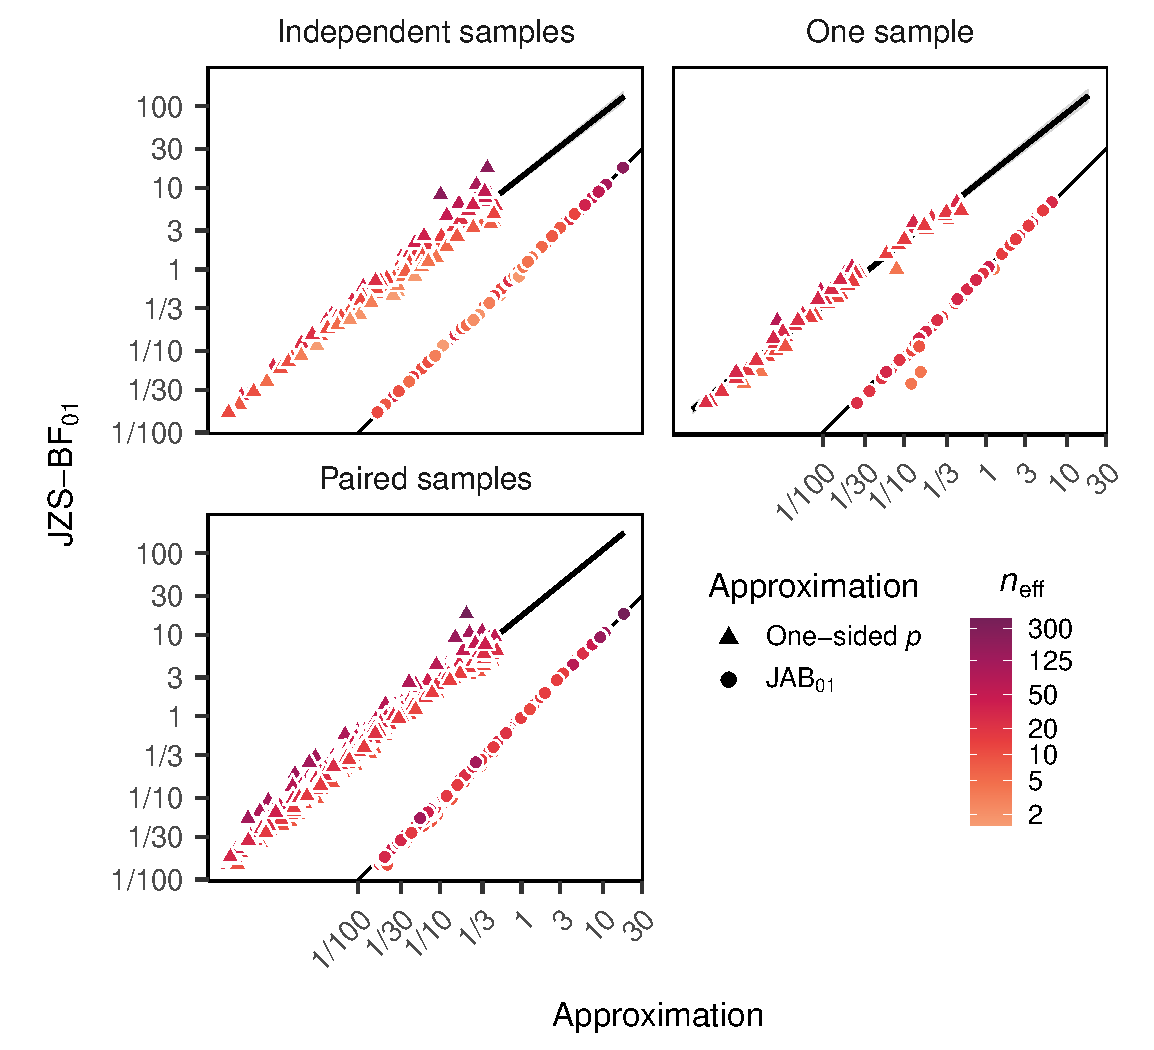
\includegraphics[keepaspectratio]{whats-in-a-p-value_files/figure-pdf/fig-jab-jzs-1.pdf}}

}

\end{figure}%

Wagenmakers (\citeproc{ref-Wagenmakers2022}{2022}) recently highlighted
that \(p\) values of single-parameter Wald tests are directly related to
Jeffreys's approximate Bayes factor (JAB; Jeffreys, 1936). Jeffreys
showed that an approximate Bayes factor can be obtained from the Wald
statistic

\[
W = \bigg [ \frac{\hat \theta - \theta_0}{\text{SE}(\hat \theta)} \bigg ]^2
\]

for a test-relevant parameter \(\theta\) and the null value \(\theta_0\)
as

\begin{equation}\phantomsection\label{eq-jab}{
\text{JAB}_{01} = A \; \sqrt{n_\text{eff}} \; \exp(-0.5 W),
}\end{equation}

where \(\sqrt{n_\text{eff}}\) is the \emph{effective sample size} that
scales the standard error (see Section~\ref{sec-appendix-n-eff}) and
\(A = [\sqrt{2 \pi}~\sigma~g(\hat \theta | \mathcal{H}_1)]^{-1}\)
depends on the prior distribution \(g()\) evaluated at the maximum
likelihood estimate of the test-relevant parameter \(\hat \theta\) and
residual standard deviation \(\sigma\). JAB relates to two-sided
\(p\)-values through the quantile function \(Q\) of the asymptotic
sampling distributions of the corresponding Wald test statistic---the
\(\chi^2(\mathrm{df} = 1)\)-distribution or the standard normal
distribution \(\mathcal{N(\mu = 0, \sigma = 1)}\),

\begin{equation}\phantomsection\label{eq-w-p}{
\begin{aligned}
W & = \phantom{[} Q_{\chi^2(1)}(1-p) \phantom{]^2} & \text{for } \chi^2\text{-tests and} \\
  & = [Q_{\mathcal{N(0,1)}}(p/2)]^2 & \text{for } z\text{-tests.}
\end{aligned}
}\end{equation}

The latter is, in words, the square of the probit-transformed one-sided
\(p\)-value. So, JAB can be understood as a transformation of the Wald
\(p\)-value using sample size that yields a principled measure of
evidence. In this way, JAB addresses the two short-comings of the
one-sided \(p\) value discussed above: It removes the bias against the
null hypothesis and takes the sample size into account. The circles in
Figure~\ref{fig-jab-jzs} illustrate that the analytic JZS-Bayes factor
with prior scale \(r = \sqrt{2}/2\) is approximated well by
corresponding JAB\footnote{Because here the \(p\)-values are from a
  \(t\)- rather than a Wald test, we use the analytic expression for the
  log likelihood ratio rather than an approximation based on \(p\)
  itself, Section~\ref{sec-appendix-llr}. With an approximate likelihood
  ratio based on the \(p\)-value (Equation~\ref{eq-w-p}), JAB
  understates the evidence against \(\mathcal{H}_0\) when effects are
  large and the effective sample size is small. Note, however, that in
  the data used here the bias exceedes a factor of 3 only in very small
  samples, Section~\ref{sec-appendix-llr}. We believe, in most
  situations, the \(p\)-based JAB is a fair approximation to the
  JZS-Bayes factor for \(t\)-tests.}. Only when the effective sample
size is very small does JAB deviate noticably from the JZS-Bayes factor.
These deviations, while noticable, are small enough to be
inconsequential. In contrast to the one-sided \(p\) value, JAB largely
accounts for differences in evidence related to sample size.

As noted above, the linear relationship between one-sided \(p\) values
and the Bayes factor shown in Figure~\ref{fig-jab-jzs} only holds for
tests of location parameters \(\mu\) in the exponential family (e.g.,
assuming normally distributed errors). When the tested hypothesis is of
a different kind, the close relationship between \(p\) and the Bayes
factor can break down. Consider the example of comparing two independent
proportions \(\theta_1\) and \(\theta_2\), where
\(\mathcal{H}_0: \theta_1 = \theta_2\). When the number of observations
is large and the probabilities not too exreme, we can test this
hypothesis using a Pearson's \(\chi^2\)-test applied to the 2 \(\times\)
2-contingency table. Another option is to reformulate the hypothesis in
terms of the odds ratio \(\text{OR}\),
\(\mathcal{H}_0: \text{OR} = \frac{\theta_1/(1-\theta_1)}{\theta_2/(1-\theta_2)} = 1\),
and test it in a logistic regression model with a binary outcome and a
binary predictor using an asymptotic \(z\)-test. Corresponding Bayesian
hypothesis tests are available (Dablander et al., 2021).

In Figure~\ref{fig-jab-prop}, we plot the results of 39 published
comparisons of two independent proportions collected by Hoekstra et
al.~(2018; reanalyzed by Dablander et al., 2021). For both hypothesis
tests there is no clear relationship between the one-sided \(p\) value
and the corresponding Bayes factors---this should not come as a
surprise. JAB, on the other hand, is closely linearly related to the
corresponding Bayes factors.

\begin{figure}

\caption{\label{fig-jab-prop}Linear relationships between Bayes factors
for point null hypotheses and \(p\)-value-based approximations for 39
results of tests comparing two proportions collected by Hoekstra et
al.~(2018; reanalyzed by Dablander et al., 2021). The top panel compares
the results of Pearson's \(\chi^2\)-test to it's Bayesian analog using
independent Beta-priors (IB); the bottom panel compares the results from
a logistic regression analysis to its Bayesian analog (LT). Triangles
represent the logarithm of the one-sided \(p\)-values, circles represent
the logarithm of \(3 p \sqrt{n}\)-JAB. The color of points indicates the
effective sample size.}

\centering{

\pandocbounded{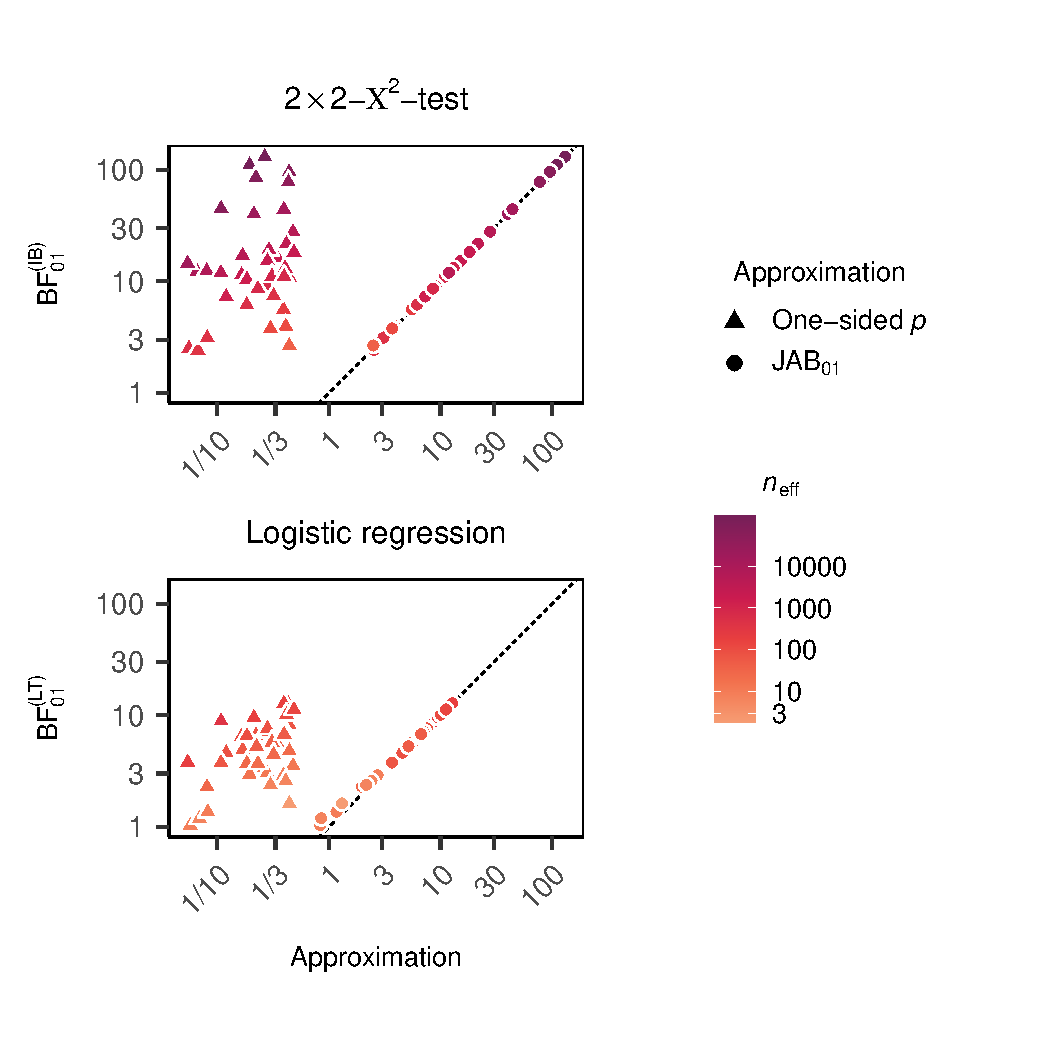
\includegraphics[keepaspectratio]{whats-in-a-p-value_files/figure-pdf/fig-jab-prop-1.pdf}}

}

\end{figure}%

These examples illustrate that JAB provides an astonishingly good
approximation to analytic Bayes factors---especially considering its
simplicity.

\subsubsection{Assumptions}\label{assumptions}

Before we use JAB to explore a prinicipled evidential interpretation of
\(p\) values, we want to highlight the assumptions underlying JAB to
clarify the boundary conditions of the approximation. JAB approximates
the Bayes factor assuming a normal likelihood,

\[
\text{BF}_{01} = \frac{\text{Pr}(\hat\theta | \mathcal{H}_0)}{\text{Pr}(\hat\theta | \mathcal{H}_1)} = \frac{\mathcal{N}(\hat\theta | \theta_0, \sigma_{\hat\theta})}{\int \mathcal{N}(\hat\theta | \theta, \sigma_{\hat\theta}) g(\theta | \mathcal{H}_1) d\theta} \approx \frac{\mathcal{N}(\hat\theta | \theta_0, \sigma_{\hat\theta})}{g(\hat\theta | \mathcal{H}_1)} = \text{JAB}_{01}.
\]

While \(\mathcal{N}(\hat\theta | \theta_0, \text{SE}(\hat\theta))\), the
density of \(\hat\theta\) under \(\mathcal{H}_0\), is known, the
integral in the denominator is not. It is assumed that this integral,
and thus,
\(\text{Pr}(\hat\theta | \mathcal{H}_1) \approx g(\hat\theta | \mathcal{H}_1)\),
that is the prior density of the maximum likelihood estimate under
\(\mathcal{H}_1\), Equation~\ref{eq-jab}. This is an asymptotic
approximation based on Laplace's approximation of the posterior
distribution of \(\theta\) (\textbf{TODO: How can I credit Samuel
here?}). Hence, the following assumptions must hold for JAB to be
accurate:

\textbf{Assumption 1}. The sampling distribution of the maximum
likelihood estimate is normally distributed,
\(\hat\theta \sim \mathcal{N}(\hat\theta, \text{SE}(\hat\theta))\). In
many cases, this assumption holds asymptotically (i.e.,
\(n_\text{eff} \to \infty\)) but it can be violated when the sampling
distribution is not normal and the sample size is small, also see
Section~\ref{sec-appendix-llr}.

\textbf{Assumption 2}. The posterior distribution is approximately
normal,
\(\theta | \hat\theta \sim \mathcal{N}(\mu_\theta, \sigma_\theta)\). In
general, the validity of this assumption depends on the model and the
prior distribution, but holds asymptotically (i.e.,
\(n_\text{eff} \to \infty\)) under quite general conditions
(Bernstein-von Mises theorem).

\textbf{Assumption 3}. The standard error is small or the prior
distribution at \(\hat\theta\) is mildly curved (concave or convex). The
standard error, of course, decreases as the effective sample size
\(n_\text{eff}\) increases. As illustrated in
Figure~\ref{fig-curvature-prior}, the curvature of the prior
distribution depends on the family of the distribution but typically
decreases as its scale increases\footnote{In small samples, it may be
  tempting to feel reassured when \(\hat\theta\) lies in the tail of the
  prior distribution where the curvature is close to 0. We caution,
  however, that the combination of small sample size and obersevations
  in the tail of the prior distribution often yields non-normal
  posterior distributions and thus violations of Assumption 2.}. Hence,
the validity of this assumption holds asymptotically or with wide,
uninformative priors. Broadly speaking, the data must be informative
relative to the prior distribution,
\(\text{SE}(\hat\theta) \ll \sigma_\theta\) (???). Otherwise JAB will be
biased against \(\mathcal{H}_0\) when \(\hat\theta\) is near the peak
and biased against \(\mathcal{H}_1\) when \(\hat\theta\) is in the tail
of the prior distribution.

\begin{figure}

\caption{\label{fig-curvature-prior}Curvature of prior distributions as
a funciton of \(\theta\) for different prior scales.}

\centering{

\pandocbounded{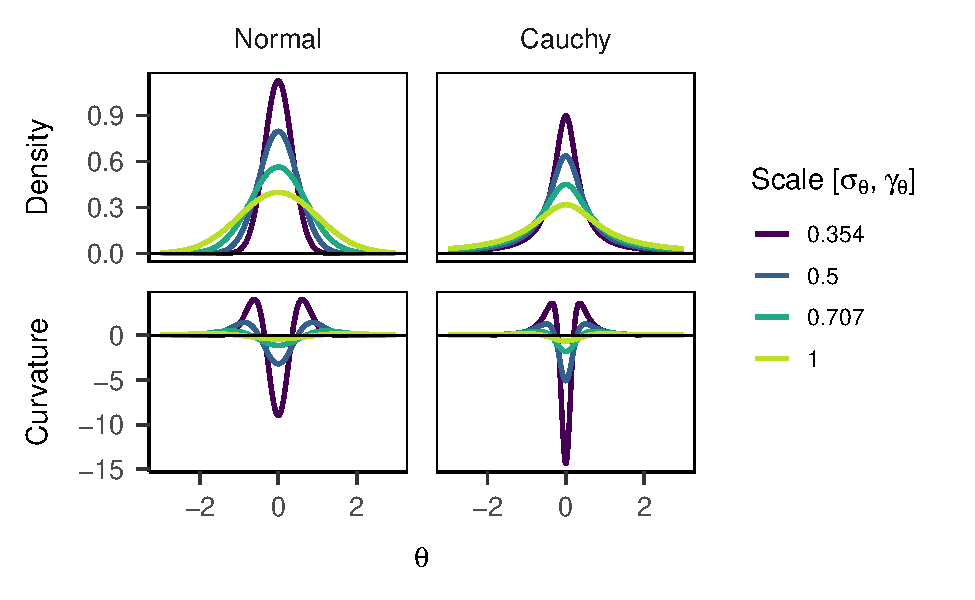
\includegraphics[keepaspectratio]{whats-in-a-p-value_files/figure-pdf/fig-curvature-prior-1.pdf}}

}

\end{figure}%

As a rule of thumb, these assumptions are likely to hold in large
samples, or for normally distributed \(\hat\theta\) if the prior
distribution is relatively wide, uninformed and places non-neglibile
mass near \(\hat\theta\). In light of this, it is remarkable how well
JAB approximates the Bayes factor in practice, Figure~\ref{fig-jab-jzs}
and Figure~\ref{fig-jab-prop}. Nonetheless, these assumptions imply that
JAB is most accurate with objective uninformed prior distributions
unless the sample size is large.

When \(W\) is calculated from \(p\) values (Equation~\ref{eq-w-p}), it
is further assumed that the \(p\) was not corrected for multiple
comparisons and was derived from a sampling distribution for a constant
sample size, see Section~\ref{sec-desirable-properties}. In practice the
latter can usually be taken for granted. With these boundary conditions
made clear, we now show how JAB offers a prinicipled evidential
interpretation of \(p\) values.

\textbf{TODO: Is there an additional assumption about nusance parameters
being uncorrelated with test parameter?}

\section{\texorpdfstring{The evidential value of
\(p\)}{The evidential value of p}}\label{the-evidential-value-of-p}

Despite repeated efforts to explain that the \(p\) value is not a
measure of evidence, proposals to treat it as such continue to be made
{[}p.~117, Bland, 2015; p.~157, Wasserman, 2004; Muff, Nilsen, O'Hara \&
Nater, 2021; Cox and Donnelly (\citeproc{ref-Cox2011}{2011}){]}.
Table~\ref{tbl-evidence-categories} lists suggested labels for grades of
evidence in favor of \(\mathcal{H}_1\) for ranges of \(p\) values. Three
things are worth noting. First, the suggested grades of evidence follow
from typical thresholds of \(p\)-values. Second, the suggested grades of
evidence are asymmetric: \(p > .100\) is said to provide ``little or no
evidence'' in favor of \(\mathcal{H}_1\); only \(p < .100\) is suggested
to carry evidential value. Third, we have shown the magnitude of the
evidence must depend on the effective sample size \(n_\text{eff}\), but
the suggested grades of evidence are independent of sample size. JAB can
be used evaluate these grades of evidence from a Bayesian perspective.

\begin{table}

{\caption{{Categorical interpreations of two-sided \(p\) values as
evidence against \(H_0\) and corresponding approximate Bayes
factors.}{\label{tbl-evidence-categories}}}
\vspace{-20pt}}

\fontsize{12.0pt}{14.4pt}\selectfont
\begin{tabular*}{\linewidth}{@{\extracolsep{\fill}}lllllll}
\toprule
 & \multicolumn{2}{c}{Grades of evidence} & \multicolumn{3}{c}{Bayesian evidence} &  \\ 
\cmidrule(lr){2-3} \cmidrule(lr){4-6}
\$p\$ & Bland (2015) & Wasserman (2004) & \$\textbackslash{}text\{JAB\}\_\{10\}(n\_\textbackslash{}text\{eff\} = 30)\$ & \$\textbackslash{}text\{JAB\}\_\{10\}(n\_\textbackslash{}text\{eff\} = 8)\$ & \$\textbackslash{}max(\textbackslash{}text\{BF\}\textasciicircum{}\{\textbackslash{}mathcal\{N\}\}\_\{10\})\$ & \$\textbackslash{}max(\textbackslash{}mathcal\{L\}\_1 / \textbackslash{}mathcal\{L\}\_0)\$ \\ 
\midrule\addlinespace[2.5pt]
\((1.000, .100]\) & Little or no evidence & Little or no evidence & \((0.18, 0.68]\) & \((0.35, 1.15]\) & \((1.00, 1.43]\) & \((1.00, 3.87]\) \\ 
\((.100, .050]\) & Weak evidence & Weak evidence & \((0.68, 1.17]\) & \((1.15, 1.90]\) & \((1.43, 2.11]\) & \((3.87, 6.83]\) \\ 
\((.050, .010]\) & Evidence & Strong evidence & \((1.17, 4.51]\) & \((1.90, 6.44]\) & \((2.11, 6.50]\) & \((6.83, 27.59]\) \\ 
\((.010, .001]\) & Strong evidence & Very strong evidence & \((4.51, 34.22]\) & \((6.44, 40.34]\) & \((6.50, 41.38]\) & \((27.59, 224.48]\) \\ 
\((.001, .000)\) & Very strong evidence &  & \((34.22, \infty)\) & \((40.34, \infty)\) & \((41.38, \infty)\) & \((224.48, \infty)\) \\ 
\bottomrule
\end{tabular*}
\begin{minipage}{\linewidth}
\(\text{JAB}_{10}\) assuming a unit-information prior centered on the test-value \(\theta_0\). \(\max(\text{BF}^{\mathcal{N}}_{10})\) is the upper limit on the evidence for \(\mathcal{H}_1\) when the prior distribution is normal {[}p. 231, @Edwards1963{]}.\\
\end{minipage}

\end{table}

Figure~\ref{fig-p-jab} A shows how \(p\) relates to Bayesian evidence as
a function of the effective sample size. As is clear form
Equation~\ref{eq-jab}, there can be no unique relationship between \(p\)
and the Bayes factor, as the latter always depends on the prior
distribution. The figure gives \(\text{JAB}_{10}\) assuming a common
prior choice in objective testing, the unit-information prior centered
on the test-value \(\theta_0\) (p.~8,
\citeproc{ref-Wagenmakers2022}{Wagenmakers, 2022}),

\begin{equation}\phantomsection\label{eq-jab-uip}{
\text{JAB}_{01} = \sqrt{n_\text{eff}} \; \exp\big[ -0.5 \; (n_\text{eff}-1) / n_\text{eff} ~~ Q_{\chi^2(1)}(1-p) \big].
}\end{equation}

This prior is sufficiently wide that results for small samples are
tenable. The solid lines represent commonly used grades of Bayesian
evidence (Jeffreys, 1961; Lee \& Wagenmakers, 2013). Note that both axes
are on log-scale.

\begin{figure}

\caption{\label{fig-p-jab}Relationship between two-sided \(p\)-value and
\(\text{JAB}_{10}\) as a function of effective sample size
\(n_\text{eff}\). Solid lines represent the \(\text{JAB}_{10}\) for a
unit-information prior centered on the test-value \(\theta_0\).
\textbf{A} Color represents the continuous evidence with the grades of
evidence suggested by Lee \& Wagenmakers (2013). The dotted lines
represent the \(\text{JAB}_{10}\) for a unit-information prior centered
on the maximum likelihood estimate \(\hat\theta\). \textbf{B}
Illustration of the shift of the grades of evidence implied by \(p\)
from small (\(n < 50\)) to large samples (\(n > 250\)).}

\centering{

\pandocbounded{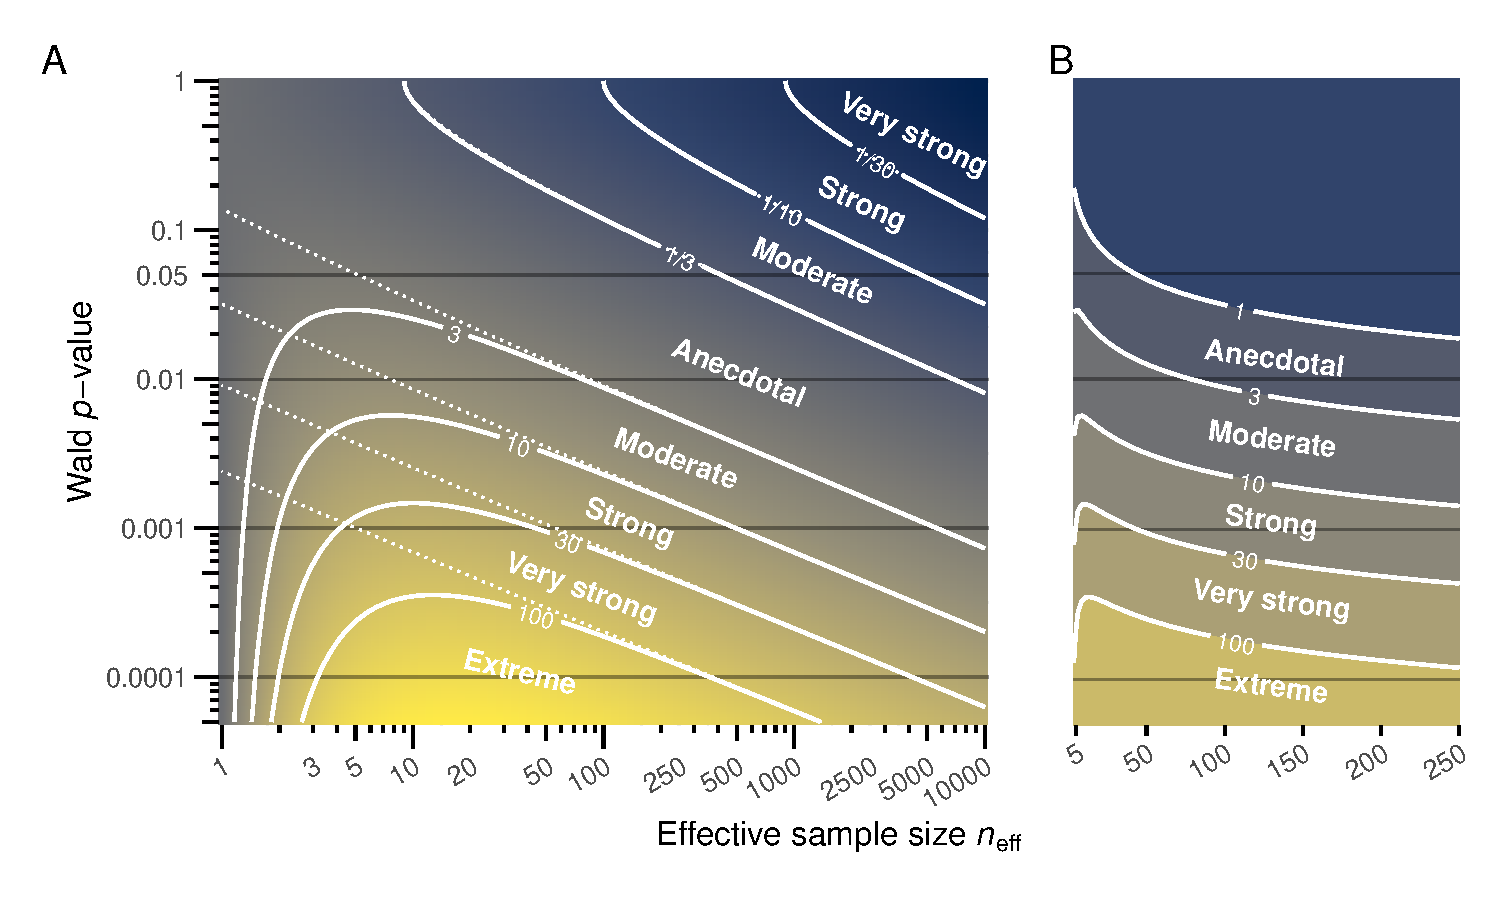
\includegraphics[keepaspectratio]{whats-in-a-p-value_files/figure-pdf/fig-p-jab-1.pdf}}

}

\end{figure}%

Several important consequences for the evidential interpration of \(p\)
follow. First, it is clear from Figure~\ref{fig-p-jab} A that a
principled interpretation of \(p\)-values as continuous measures of
evidence must take the effective sample size into account. The grades of
evidence suggested by Bland (2015) approximately correspond to the
Bayesian grades of evidence suggested by Lee \& Wagenmakers (2013), if
the effective sample size is \(n_\text{eff} \approx 8\). This is,
however, close to the upper bound on the evidence for this class of
prior distribution, \(\max(\text{BF}^{\mathcal{N}}_{10})\) (p.~231,
\citeproc{ref-Edwards1963}{Edwards et al., 1963}),
Table~\ref{tbl-evidence-categories}. As \(n_\text{eff}\) increases (or
decrease), the suggested grades quickly overstate the Bayesian evidence
for \(\mathcal{H}_1\). The grades of evidence suggested by Wasserman
(2004) overstate the Bayesian evidence even when
\(n_\text{eff} \approx 8\)---even though Wasserman
(\citeproc{ref-Wasserman2000}{2000}) agrees with the grades of Bayesian
evidence suggested by Lee \& Wagenmakers (2013). For \(p < .10\) and
\(n_\text{eff} > 20\), as the effective sample size increases
\(\log(p)\) must decreases approximately linearly to yield constant
evidence (Benjamin et al., XXXX). Hence, changes in effective sample
size noticably affect the evidence in \(p\) in small samples, but are
less consequential in larger samples, Figure~\ref{fig-p-jab} B. Muff,
Nilsen, O'Hara and Nater (2021) argue that this deceleration renders
sample size irrelevant for the evidential interpretation of \(p\)
suggested by Bland (2015). Figure~\ref{fig-p-jab} B shows this to be
incorrect (also see Hartig \& Barraquand, 2022). Assume that typical
samples in their field of research are large enough that changing the
sample size changes the evidence neglibably,
e.g.~\(n_\text{eff} > 300\). At this point Bland's grades of evidence
overstate the evidence for \(\mathcal{H}_1\). For example, in small
samples (\(n_\text{eff} < 20\)) \(.01 < p < .001\) usually implies
moderate to very strong evidence for \(\mathcal{H}_1\), but in larger
samples (\(n_\text{eff} = 300\)) this evidence is strong at best but
usually anecdotal or moderate. In other words, the evidence for
\(\mathcal{H}_1\) is shifted down relative to Bland's by a full grade.

Second, given \(p\) implies less evidence for \(\mathcal{H}_1\) as the
effective sample size increases, but in small samples this trend
typically reverses. As shown in Figure~\ref{fig-p-jab} B and highlighted
in Figure~\ref{fig-p-jab} A, when the unit-information prior is centered
on the test value \(\theta_0\), the evidence for \(\mathcal{H}_1\)
implied by \(p\) levels off and decreases as the effective sample size
becomes very small, \(n_\text{eff} < 8\). However, as shown by the
dotted curves in Figure~\ref{fig-p-jab} A, when the prior is centered on
the maximum likelihood estimate \(\hat\theta\), the evidence for
\(\mathcal{H}_1\) continous to increase with the effective sample size.
The difference is most prominent in small samples. The same prior
underlies another popular approximation to the Bayes factor, the
\(\text{BIC}\). Again, this prior distribution amounts to using the data
twice and is best considered a lower bound on the Bayes factor for the
unit-information prior, in particular in small samples
\(n_\text{eff} < 30\) (Held \& Ott, 2018).

A third important consequence that evident from Figure~\ref{fig-p-jab} A
pertains to the evidence implied by \(p > 0.1\). In line with Bland
(2015) and Wasserman (2004), in very small samples
(\(n_\text{eff} < 9\)) such results provides little or no evidence for
either \(\mathcal{H}_1\) or \(\mathcal{H}_0\). However, this is not true
in general. In moderate (\(9 < n_\text{eff} < 100\)) and large samples
(\(100 < n_\text{eff} < 900\)) it is possible to obtain moderate to
strong evidence for \(\mathcal{H}_0\)! Hence, in sufficiently large
samples \$.1 \textless{} p \textless{} 1 \$ can be informative and
provide meaningful evidence for the absence of an effect.

Lastly, JAB can be used to derive lower and upper bounds on the Bayes
factor. For simplicity, consider a unit-information prior centered on
the maximum likelihood estimate \(\hat\theta\), i.e., \(A = 1\) in
Equation~\ref{eq-jab}. Note that, while mathematically convenient, a
prior distribution centered on \(\hat\theta\) amounts to using the data
twice (to inform the prior distribution under \(\mathcal{H}_1\) and to
test this hypothesis) and will bias the evidence in favor of
\(\mathcal{H}_1\). It can in itself be considered a lower bound on Bayes
factors for the unit-information prior. The lower bound on this Bayes
factor for a given \(p\) is reached when \(n_\text{eff} = 1\),

\[
\min(\text{JAB}_{01}) = \exp\left[-0.5~\left[Q_{\mathcal{N(0,1)}}(p/2)\right]^2\right].
\]

This is the lower bound on the likelihood ratio
{[}\(\max(\mathcal{L}_0 / \mathcal{L}_1)\); p.~228, Edwards et al.
(\citeproc{ref-Edwards1963}{1963}); p.~116 Berger and Sellke
(\citeproc{ref-Berger1987}{1987}){]},
Table~\ref{tbl-evidence-categories}. For a comprehensive review on other
lower bounds on the Bayes factor see the comprehensive review by Held
and Ott (\citeproc{ref-Held2018}{2018}). Conversely, the upper bound on
the evidence for \(\mathcal{H}_0\) for a given effective sample size
\(n_\text{eff}\) is reached when \(p \to 1\) and thus

\[
\max(\text{JAB}_{01}) = \sqrt{n_\text{eff}}.
\]

This simple expression holds regardless of the center of the
unit-information prior and is a useful reference point when evaluating
claims about the absence of an effect based on a non-significant NHST.
Bounds can similary be derived for other prior distributions.

\section{Conclusion}\label{conclusion}

Interpreting \(p\) values as a measure of statistical evidence for a
hypothesis is suggested in statistics text books (p.~117, Bland, 2015;
p.~157, Wasserman, 2004; Cox and Donnelly
(\citeproc{ref-Cox2011}{2011})) and continues to be pervasive in
research practice (Gigerenzer, \textless{}Gigerenzer
(\citeproc{ref-Gigerenzer2018}{2018})\textgreater; \textless{}Cohen
(\citeproc{ref-Cohen1994}{1994})\textgreater). Calls to abandon this
practice {[}e.g., \textbf{???}, Hubbard and Lindsay
(\citeproc{ref-Hubbard2008}{2008}); Royall, 1997; Goodman \& Royall,
1988{]} have had limited success. We hope our discussion contributes to
educating researchers about the limitations of \(p\) values, but we
realize that education alone is not effective in changing behavior
(\citeproc{ref-Albarracn2024}{Albarracín et al., 2024};
\citeproc{ref-Wood2024}{Wood, 2024}). Instead of just asking someone to
quit a bad habit, it is sometimes more effective to offer them a better
alternative (\citeproc{ref-Albarracn2024}{Albarracín et al., 2024}). But
adopting better alternatives is difficult when they add friction and
\(p\) values are often much easier to calculate than Bayes factors. So
in this paper, we provide a simple formula to transform \(p\) values
into an approximate measure of evidence requiring only the effective
sample size: Jeffreys's approximate Bayes factor {[}JAB; Jeffreys, 1936;
Wagenmakers (\citeproc{ref-Wagenmakers2022}{2022}){]},
Equation~\ref{eq-jab}. We have demonstrated that JAB is a surprisingly
good approximation to the Bayes factors from objective tests of mean
comparisons and proportions across a range of realistic scenarios,
Figure~\ref{fig-jab-jzs} and Figure~\ref{fig-jab-prop}. And we have
illustrated how the evidence implied by a \(p\) value is not constant
but depends on the effective sample size, Figure~\ref{fig-p-jab}.

We believe that JAB and Figure~\ref{fig-p-jab} can be useful tools for
researchers, reviewers, and readers to assess claims of both presence
and absence of effects---regardless of whether the data were peaked at
during data collection. And in case Equation~\ref{eq-jab-uip} still
causes too much friction, Wagenmakers
(\citeproc{ref-Wagenmakers2022}{2022}) has suggested an even simpler
approximation, where
\(\text{JAB}_{01} \approx 3 p \sqrt{n_\text{eff}}\), if \(p \leq .10\)
(their Eq. 9).

\clearpage

\section{References}\label{references}

\phantomsection\label{refs}
\begin{CSLReferences}{1}{0}
\bibitem[\citeproctext]{ref-Albarracn2024}
Albarracín, D., Fayaz-Farkhad, B., \& Granados Samayoa, J. A. (2024).
Determinants of behaviour and their efficacy as targets of behavioural
change interventions. \emph{Nature Reviews Psychology}, \emph{3}(6),
377--392. \url{https://doi.org/10.1038/s44159-024-00305-0}

\bibitem[\citeproctext]{ref-Allabadi2024}
Al-Labadi, L., Alzaatreh, A., \& Evans, M. (2024). \emph{How to measure
evidence and its strength: Bayes factors or relative belief ratios?}
\url{https://doi.org/10.48550/arXiv.2301.08994}

\bibitem[\citeproctext]{ref-Bartos2024}
Bartoš, F., Sarafoglou, A., Godmann, H. R., Sahrani, A., Leunk, D. K.,
Gui, P. Y., Voss, D., Ullah, K., Zoubek, M. J., Nippold, F., Aust, F.,
Vieira, F. F., Islam, C.-G., Zoubek, A. J., Shabani, S., Petter, J.,
Roos, I. B., Finnemann, A., Lob, A. B., \ldots{} Wagenmakers, E.-J.
(2024). \emph{Fair coins tend to land on the same side they started:
Evidence from 350,757 flips}.
\url{https://doi.org/10.48550/ARXIV.2310.04153}

\bibitem[\citeproctext]{ref-Beal1987}
Beal, S. L. (1987). Asymptotic confidence intervals for the difference
between two binomial parameters for use with small samples.
\emph{Biometrics}, \emph{43}(4), 941.
\url{https://doi.org/10.2307/2531547}

\bibitem[\citeproctext]{ref-Berger2013}
Berger, J. O., Bayarri, M. J., \& Pericchi, L. R. (2013). The effective
sample size. \emph{Econometric Reviews}, \emph{33}(1--4), 197--217.
\url{https://doi.org/10.1080/07474938.2013.807157}

\bibitem[\citeproctext]{ref-Berger1987}
Berger, J. O., \& Sellke, T. (1987). Testing a point null hypothesis:
The irreconcilability ofP-values and evidence. \emph{Journal of the
American Statistical Association}, \emph{82}(397), 112--122.
\url{https://doi.org/10.1080/01621459.1987.10478397}

\bibitem[\citeproctext]{ref-Cohen1994}
Cohen, J. (1994). The earth is round (p \textless{} .05). \emph{American
Psychologist}, \emph{49}(12), 997--1003.
\url{https://doi.org/10.1037/0003-066x.49.12.997}

\bibitem[\citeproctext]{ref-Cole2020}
Cole, S. R., Edwards, J. K., \& Greenland, S. (2020). Surprise!
\emph{American Journal of Epidemiology}, \emph{190}(2), 191--193.
\url{https://doi.org/10.1093/aje/kwaa136}

\bibitem[\citeproctext]{ref-Cox2011}
Cox, D. R., \& Donnelly, C. A. (2011). \emph{Principles of applied
statistics}. Cambridge University Press.
\url{https://doi.org/10.1017/cbo9781139005036}

\bibitem[\citeproctext]{ref-Edwards1963}
Edwards, W., Lindman, H., \& Savage, L. J. (1963). Bayesian statistical
inference for psychological research. \emph{Psychological Review},
\emph{70}(3), 193--242. \url{https://doi.org/10.1037/h0044139}

\bibitem[\citeproctext]{ref-Etz2017}
Etz, A., Gronau, Q. F., Dablander, F., Edelsbrunner, P. A., \&
Baribault, B. (2017). How to become a bayesian in eight easy steps: An
annotated reading list. \emph{Psychonomic Bulletin \&Amp; Review},
\emph{25}(1), 219--234. \url{https://doi.org/10.3758/s13423-017-1317-5}

\bibitem[\citeproctext]{ref-Francis2016}
Francis, G. (2016). Equivalent statistics and data interpretation.
\emph{Behavior Research Methods}, \emph{49}(4), 1524--1538.
\url{https://doi.org/10.3758/s13428-016-0812-3}

\bibitem[\citeproctext]{ref-Francis2022}
Francis, G., \& Jakicic, V. (2022). Equivalent statistics for a
one-sample t-test. \emph{Behavior Research Methods}, \emph{55}(1),
77--84. \url{https://doi.org/10.3758/s13428-021-01775-3}

\bibitem[\citeproctext]{ref-Gigerenzer2018}
Gigerenzer, G. (2018). Statistical rituals: The replication delusion and
how we got there. \emph{Advances in Methods and Practices in
Psychological Science}, \emph{1}(2), 198--218.
\url{https://doi.org/10.1177/2515245918771329}

\bibitem[\citeproctext]{ref-Greenland2019}
Greenland, S. (2019). Valid p-values behave exactly as they should: Some
misleading criticisms of p-values and their resolution with s-values.
\emph{The American Statistician}, \emph{73}(sup1), 106--114.
\url{https://doi.org/10.1080/00031305.2018.1529625}

\bibitem[\citeproctext]{ref-Held2018}
Held, L., \& Ott, M. (2018). On p-values and bayes factors. \emph{Annual
Review of Statistics and Its Application}, \emph{5}(1), 393--419.
\url{https://doi.org/10.1146/annurev-statistics-031017-100307}

\bibitem[\citeproctext]{ref-Hubbard2008}
Hubbard, R., \& Lindsay, R. M. (2008). Why p values are not a useful
measure of evidence in statistical significance testing. \emph{Theory
\&Amp; Psychology}, \emph{18}(1), 69--88.
\url{https://doi.org/10.1177/0959354307086923}

\bibitem[\citeproctext]{ref-Kruschke2014}
Kruschke, J. (2014). \emph{Doing bayesian data analysis - a tutorial
with r, JAGS, and stan}. Academic Press.

\bibitem[\citeproctext]{ref-Lakens2022}
Lakens, D. (2022). \emph{Improving your statistical inferences}. Zenodo.
\url{https://doi.org/10.5281/ZENODO.6409077}

\bibitem[\citeproctext]{ref-Marsman2016}
Marsman, M., \& Wagenmakers, E.-J. (2016). Three insights from a
bayesian interpretation of the one-sided p value. \emph{Educational and
Psychological Measurement}, \emph{77}(3), 529--539.
\url{https://doi.org/10.1177/0013164416669201}

\bibitem[\citeproctext]{ref-Morey2016}
Morey, R. D., Romeijn, J.-W., \& Rouder, J. N. (2016). The philosophy of
bayes factors and the quantification of statistical evidence.
\emph{Journal of Mathematical Psychology}, \emph{72}, 6--18.
\url{https://doi.org/10.1016/j.jmp.2015.11.001}

\bibitem[\citeproctext]{ref-Murtaugh2014}
Murtaugh, P. A. (2014). In defense of p values. \emph{Ecology},
\emph{95}(3), 611--617. \url{https://doi.org/10.1890/13-0590.1}

\bibitem[\citeproctext]{ref-Perezgonzalez2015}
Perezgonzalez, J. D. (2015). P-values as percentiles. Commentary on:
"Null hypothesis significance tests. A mix-up of two different theories:
The basis for widespread confusion and numerous misinterpretations".
\emph{Frontiers in Psychology}, \emph{6}.
\url{https://doi.org/10.3389/fpsyg.2015.00341}

\bibitem[\citeproctext]{ref-Rafi2020}
Rafi, Z., \& Greenland, S. (2020). Semantic and cognitive tools to aid
statistical science: Replace confidence and significance by
compatibility and surprise. \emph{BMC Medical Research Methodology},
\emph{20}(1). \url{https://doi.org/10.1186/s12874-020-01105-9}

\bibitem[\citeproctext]{ref-Wagenmakers2022}
Wagenmakers, E.-J. (2022). \emph{Approximate objective bayes factors
from p-values and sample size: The 3p√n rule}.
\url{https://doi.org/10.31234/osf.io/egydq}

\bibitem[\citeproctext]{ref-Wasserman2000}
Wasserman, L. (2000). Bayesian model selection and model averaging.
\emph{Journal of Mathematical Psychology}, \emph{44}(1), 92--107.
\url{https://doi.org/10.1006/jmps.1999.1278}

\bibitem[\citeproctext]{ref-Wilks1938}
Wilks, S. S. (1938). The large-sample distribution of the likelihood
ratio for testing composite hypotheses. \emph{The Annals of Mathematical
Statistics}, \emph{9}(1), 60--62.
\url{https://doi.org/10.1214/aoms/1177732360}

\bibitem[\citeproctext]{ref-Wood2024}
Wood, W. (2024). Habits, goals, and effective behavior change.
\emph{Current Directions in Psychological Science}, \emph{33}(4),
226--232. \url{https://doi.org/10.1177/09637214241246480}

\end{CSLReferences}

\clearpage

\appendix

\section{\texorpdfstring{What is
\(n_\text{eff}\)?}{What is n\_\textbackslash text\{eff\}?}}\label{sec-appendix-n-eff}

In the main text, we largely glossed over an imporant issue when
calculating JAB: What is the effective sample size \(n_\text{eff}\) in
Equation~\ref{eq-jab}? The term \(\sqrt{n_\text{eff}}\) is the
denominator of the standard error of the maximum likelihood estimate,
\(\text{SE}(\hat \theta)\)---it is a function of sample size and scales
the standard deviation of the sampling distribution of the
\(\hat \theta\). Hence, the correct definition of \(n_\text{eff}\)
depends on \(\theta\). Berger et al. (\citeproc{ref-Berger2013}{2013})
provide a general treatment of effective sample size in the linear model
for the BIC but equally applies to JAB. In the following, we show a
simpler derivation for the applications shown in in
Figure~\ref{fig-jab-jzs} and Figure~\ref{fig-jab-prop}.

\subsection{\texorpdfstring{Effective sample size for one-sample
\(t\)-tests}{Effective sample size for one-sample t-tests}}\label{effective-sample-size-for-one-sample-t-tests}

In the case of a one-sample \(t\)-test, \(\hat \theta = \hat \mu\)---the
sample mean---and the standard error is
\(\text{SE}(\hat \theta = \hat \mu) = \hat \sigma / \sqrt{n}\). Here,
the effective sample size is simply the number of observations,
\(n_\text{eff} = n\). Similarly, in the paired-sample \(t\)-test,
\(\hat \theta = \hat \mu_\Delta\)---the sample mean of the differences
between the paired observations---and the standard error is
\(\text{SE}(\hat \theta = \hat \mu_\Delta) = \hat \sigma_\Delta / \sqrt{n_\Delta}\).
Now, the effective sample size is the number of differences or,
equivalently, the number of pairs, \(n_\text{eff} = n_\Delta\). In the
independent sample \(t\)-test,
\(\hat \theta = \hat \mu_1 - \hat \mu_2 = \Delta \hat \mu\)---the
difference between the sample means---and, assuming homogeneous
variances, the standard error is based on pooled estimate of the
standard deviation. In this case, the effective sample size is half the
harmonic mean \(H\) of the sample sizes,

\[
n_\text{eff} = H(n_1, n_2) / 2 = (n_2~n_1) / (n_1 + n_2),
\]

an average dominated by the smaller sample size. In balanced designs,
where \(n_1 = n_2\), this expression simplifies to
\(n_\text{eff} = (n_1 + n_2) / 4\), the arithmetic mean. For the
interested reader, we provide the equations for the effective sample
size in the more general case of unequal variances---Welch's
\(t\)-test---and the tests of independent proportions in below. To
summarize, the \(n_\text{eff}\) in JAB is the factor that scales the
standard error of \(\hat \theta\) and is a \emph{function} of sample
size. \(n_\text{eff}\) is calculated differently for each model and
parameterization. Determining the correct \(n_\text{eff}\) can be
difficult in more complex models, which is why

\subsection{\texorpdfstring{Effective sample size for independent-sample
\(t\)-tests}{Effective sample size for independent-sample t-tests}}\label{effective-sample-size-for-independent-sample-t-tests}

In the independent sample \(t\)-test,
\(\hat \theta = \hat \mu_1 - \hat \mu_2 = \Delta \hat \mu\)---the
difference between the sample means---and the standard error is

\[
\begin{aligned}
\text{SE}(\hat \theta = \Delta \hat \mu) & = \hat \sigma_p \cdot \sqrt{1/n_1 + 1/n_2} \\
& = \hat \sigma_p \cdot \sqrt{(n_1 + n_2) / (n_1 \cdot n_2)} \\
& = \frac{ \hat \sigma_p }{ \sqrt{(n_1 \cdot n_2) / (n_1 + n_2)}},
\end{aligned}
\]

where \(\hat \sigma_p\) is the pooled estiamte of the standard
deviation, i.e.~the assumedly \emph{common} standard deviation estimated
using the data from both samples. So here, the effective sample size
\(n_\text{eff}\) is half the harmonic mean of the two sample sizes,

\[
n_\text{eff} = 0.5 \cdot H(n_1, n_2) = (n_1 \cdot n_2) / (n_1 + n_2),
\]

an average dominated by the smaller sample size. When the variance are
unequal, and Welch's \(t\)-test is reported, the standard error is based
on separate estimates of the standard deviation,

\[
\text{SE}(\hat \theta = \Delta \hat \mu) = \sqrt{\hat \sigma_1^2 / n_1 + \hat \sigma_2^2 / n_2}.
\]

To obtain the effective sample size in the above form, we define a
variance ratio \(w = s^2_1/s^2_2\), which yields

\[
\begin{aligned}
\text{SE}(\hat \theta = \Delta \hat \mu) & = \hat \sigma_1 \cdot \sqrt{1 / n_1 + w / n_2} \\
& = \hat \sigma_1 \cdot \sqrt{(n_1 + wn_2) / (n_1 \cdot n_2)} \\
& = \frac{ \hat \sigma_1 }{ \sqrt{(n_1 \cdot n_2) / (n_1 + wn_2)}}.
\end{aligned}
\]

Hence, \(n_\text{eff} = (n_1 \cdot n_2) / (n_1 + wn_2)\), which is half
of harmonic mean of the sample sizes weighted by the variance ratio
\(w\).

See Berger et al. (\citeproc{ref-Berger2013}{2013}) for more general
derivation of the effective sample size in the linear model.

\subsection{Effective sample size for two independent
proportions}\label{effective-sample-size-for-two-independent-proportions}

For the test of log odds ratio the standard error can be calculated from
the cell frequencies as,

\[
\text{SE}(\hat{\theta} = \log{\text{OR}}) = \sqrt{\frac{1}{y_1 + 0.5} + \frac{1}{y_2 + 0.5} + \frac{1}{n_1 - y_1 + 0.5} + \frac{1}{n_2 - y_2 + 0.5}},
\]

(e.g., Anscombe, 1956; Gart, 1966; Haldane, 1956; cf.~Agresti, 1999)
which implies that the effective sample size for JAB is,

\[
n_\text{eff} = \left(\frac{1}{y_1} + \frac{1}{y_2} + \frac{1}{n_1 - y_1} + \frac{1}{n_2 - y_2}\right)^{-1}.
\]

For the \(\chi^2\)-test, the effective sample size can be derived from
the formula for the confidence interval of the difference between two
proportions (\citeproc{ref-Beal1987}{Beal, 1987}),

\[
n_\text{eff} = \left[\frac{\hat{\pi}_1(1-\hat{\pi}_1)}{n_1} + \frac{\hat{\pi}_2(1-\hat{\pi}_2)}{n_2}\right]^{-1}.
\]

\section{\texorpdfstring{\(p\)-based JAB for independent and dependent
sample
\(t\)-tests}{p-based JAB for independent and dependent sample t-tests}}\label{sec-appendix-llr}

In Equation~\ref{eq-jab}, \(W\) is used to approximate the likelihood
ratio (Wilk's theorem, \citeproc{ref-Wilks1938}{Wilks, 1938}), i.e., as
\(n \to \infty\)

\[
\begin{aligned}
W + o_p(1) & = -2 \log(\mathcal{L}_{0} / \mathcal{L}_{1}) \text{, so that} \\
\exp(-0.5 W) + o_p(1) & = \mathcal{L}_{0} / \mathcal{L}_{1}.
\end{aligned}
\]

Equation~\ref{eq-w-p} shows that the Wald statistic \(W\) can be
calculated from it's corresponding \(p\)-value. However, the
\(p\)-values shown in Figure~\ref{fig-jab-jzs} based on \(t\)-values
with varying degrees of freedom. When we use these \(p\)-values to
calculate JAB, we deviate from the original derivation of JAB in two
ways: (1) The underlying \(t\)-statistic is based on a standard error
that relies on the unbiased estimate of the population variance
(Bessel's correction, \(n - 1\)). The Wald statistic, however, is based
on the uncorrected maximum likelihood estimate of the variance. (2) The
\(p\)-value is based on the \(t\)-distribution rather than the standard
normal distribution. Figure~\ref{fig-jabp-jzs} illustrates the
consequences of these deviations. JAB overstates the evidence for
\(\mathcal{H}_1\) when \(n_\text{eff}\) is small. Note, however, that in
the data used here the bias exceedes a factor of 3 only in very small
samples. We thus believe, in most situations, the \(p\)-based JAB is a
fair approximation to the JZS-Bayes factor for \(t\)-tests. To quote
Jeffreys (1961), another influential Bayesian statistician, on the
precision of Bayes factors:

\begin{quote}
it will seldom matter appreciably to further procedure if {[}the Bayes
factor{]} is wrong by as much as a factor of 3. (p.~433)
\end{quote}

\begin{figure}

\caption{\label{fig-jabp-jzs}Linear relationships between analytic
JZS-Bayes factors for point null hypotheses and \(p\)-value-based JAB
for 704 \(t\)-test results collected by Aczel et al.~(2018) and Wetzels
et al.~(2011). Triangles represent the logarithm of the one-sided
\(p\)-values, circles represent the logarithm of \(\text{JAB}_{01}\).
The color of points indicates the effective sample size. The thick solid
black line shows the estimated linear relationship between the one-sided
\(p\) values and the JZS-Bayes factor. The grey area shows the margin of
error of a factor of 3 (p.~433, Jeffreys, 1961).}

\centering{

\pandocbounded{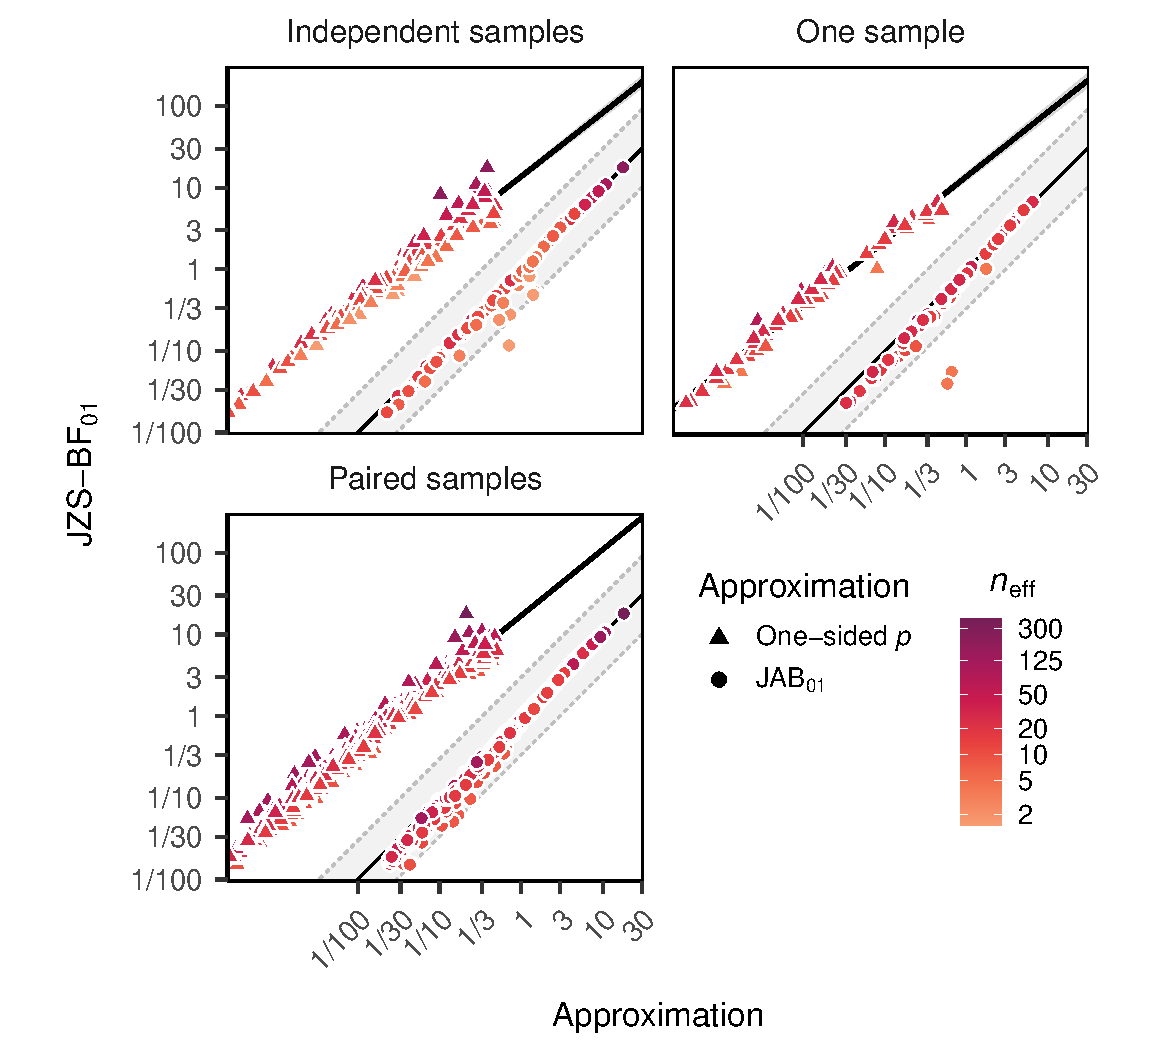
\includegraphics[keepaspectratio]{whats-in-a-p-value_files/figure-pdf/fig-jabp-jzs-1.pdf}}

}

\end{figure}%

The results shown in Figure~\ref{fig-jabp-jzs} rely on the exact
likelihood ratio, which can be calculated from the \(t\)-value
{[}Kendall \& Stuart, 1961; Murtaugh
(\citeproc{ref-Murtaugh2014}{2014}); Francis and Jakicic
(\citeproc{ref-Francis2022}{2022}); Francis
(\citeproc{ref-Francis2016}{2016}){]},

\[
\log(\mathcal{L}_{1} / \mathcal{L}_{0}) = \frac{N}{2}\log\bigg(1 + \frac{t^2}{N - k}\bigg),
\]

where \(N\) is the total sample size and \(k\) is the number of samples.
The term \(N - k\) represents the residual degrees of freedom, which
serve as Bessel's correction for the unbiased estimate of the population
variance. As noted above, this is necessary because the likelihood ratio
is based on the uncorrected maximum likelihood estimate of the variance.
We have found that the likelihood ratio approximation based on \(p\) can
yield even better results if the approximate \(W\) is adjusted by a
corrective factor of \((N / (N - k))\), where \(N\) is the total sample
size and \(k\) is the number of samples:

\[
\begin{aligned}
W_t & = \left[Q_{\mathcal{N(0,1)}}(p_t/2)\right]^2 \\
   & \approx \frac{(\hat \theta - \theta_0)^2}{\sum{(\theta_i - \theta_0)^2} / [(N - k) \; n_\text{eff}]} \\ \\
W & \approx W_t \frac{N}{N - k} \\
  & \approx \frac{(\hat \theta - \theta_0)^2}{\sum{(\theta_i - \theta_0)^2} / [N \; n_\text{eff}]},
\end{aligned}
\]

and

\[
\text{JAB}_{01} \approx A \; \sqrt{n_\text{eff}} \; \exp\left(-0.5 W_t\right)^{N/(N - k)}.
\]

The correction yields a \(t\) statistic calculated from the maximum
likelihood estimate of the variance. This statistic is known to follow a
location-scale \(t\) distribution with
\(t(\mu = 0, \tau^2 = N / (N - k), \nu = N - k)\). Knowing that
\(t(\nu = n - 1) \xrightarrow[]{D} \mathcal{N}(\mu = 0, \sigma^2 = 1)\)
as \(n \to \infty\), we see that the location-scale \(t\) distribution,
too, converges to the standard normal distribution as the sample size
increases. Figure~\ref{fig-bf-t-z} shows the bias in JAB for a
one-sample \(t\)-test when \(W\) approximated from \(p\), with and
without the correction, relative to the analytic likelihood ratio. Both
approximations work well even in relatively small samples---\(n > 10\)
and \(n > 5\), respectively---and in particular for \(p > .05\).

\begin{figure}

\caption{\label{fig-bf-t-z}Bias of likelihood ratio approximations from
\(p\) of a one-sample \(t\)-test (\(W_t\); left panel) and with
additional correction (\(N / (N - 1)\); right panel). The grey area
shows the margin of error of a factor of 3 (p.~433, Jeffreys, 1961).}

\centering{

\pandocbounded{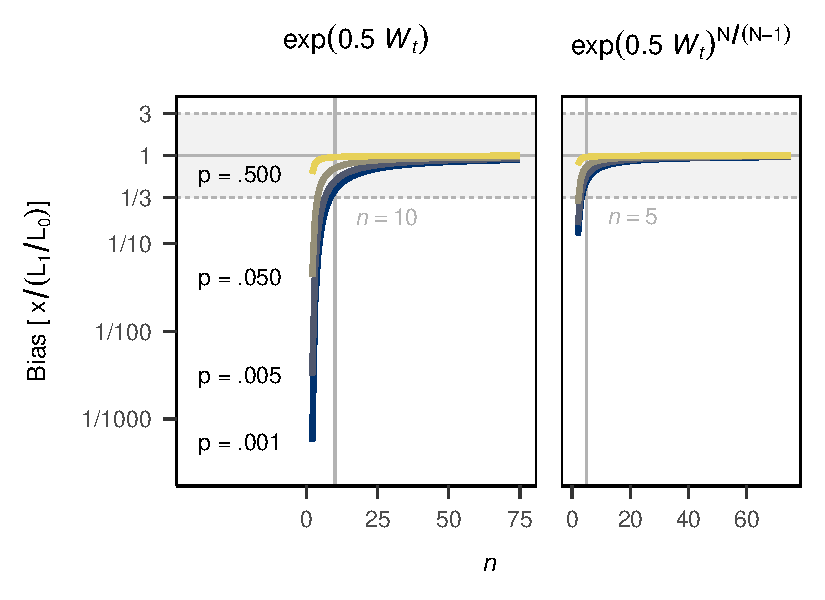
\includegraphics[keepaspectratio]{whats-in-a-p-value_files/figure-pdf/fig-bf-t-z-1.pdf}}

}

\end{figure}%

When used to calculate JAB, the corrective factor should also be applied
to the standard error,

\[
\text{SE}(\hat \theta) \approx \sqrt{[\text{SE}_t(\hat \theta)]^2 \frac{N}{N - k}}.
\]






\end{document}
